%%%%%%%%%%%%%%%%%%%%%%%%%%%%%%%%%%%%%%%%%
% Jacobs Landscape Poster
% LaTeX Template
% Version 1.1 (14/06/14)
%
% Created by:
% Computational Physics and Biophysics Group, Jacobs University
% https://teamwork.jacobs-university.de:8443/confluence/display/CoPandBiG/LaTeX+Poster
% 
% Further modified by:
% Nathaniel Johnston (nathaniel@njohnston.ca)
%
% This template has been downloaded from:
% http://www.LaTeXTemplates.com
%
% License:
% CC BY-NC-SA 3.0 (http://creativecommons.org/licenses/by-nc-sa/3.0/)
%
%%%%%%%%%%%%%%%%%%%%%%%%%%%%%%%%%%%%%%%%%

%----------------------------------------------------------------------------------------
%	PACKAGES AND OTHER DOCUMENT CONFIGURATIONS
%----------------------------------------------------------------------------------------

\documentclass[final]{beamer}

\usepackage[scale=1.24]{beamerposter} % Use the beamerposter package for laying out the poster
\usepackage{amsmath}
\usepackage{mathrsfs}
\usepackage{ upgreek }
\usepackage[T1]{fontenc}
\usepackage[utf8]{inputenc}
\usepackage{ bbold }
\usepackage{dsfont}
\usepackage{array}
\usepackage{mathtools, bm}
\usepackage{amssymb, bm}
\usepackage{amsthm} 
\usepackage{geometry} 
\usepackage{relsize,exscale}
\usepackage{multicol}

\usetheme{confposter} % Use the confposter theme supplied with this template

\setbeamercolor{block title}{fg=ngreen,bg=white} % Colors of the block titles
\setbeamercolor{block body}{fg=black,bg=white} % Colors of the body of blocks
\setbeamercolor{block alerted title}{fg=white,bg=dblue!70} % Colors of the highlighted block titles
\setbeamercolor{block alerted body}{fg=black,bg=dblue!10} % Colors of the body of highlighted blocks
% Many more colors are available for use in beamerthemeconfposter.sty

%-----------------------------------------------------------
% Define the column widths and overall poster size
% To set effective sepwid, onecolwid and twocolwid values, first choose how many columns you want and how much separation you want between columns
% In this template, the separation width chosen is 0.024 of the paper width and a 4-column layout
% onecolwid should therefore be (1-(# of columns+1)*sepwid)/# of columns e.g. (1-(4+1)*0.024)/4 = 0.22
% Set twocolwid to be (2*onecolwid)+sepwid = 0.464
% Set threecolwid to be (3*onecolwid)+2*sepwid = 0.708

\newlength{\sepwid}
\newlength{\onecolwid}
\newlength{\twocolwid}
\newlength{\threecolwid}
\setlength{\paperwidth}{36in} % A0 width: 46.8in
\setlength{\paperheight}{48in} % A0 height: 33.1in
\setlength{\sepwid}{0.024\paperwidth} % Separation width (white space) between columns
\setlength{\onecolwid}{0.22\paperwidth} % Width of one column
\setlength{\twocolwid}{0.464\paperwidth} % Width of two columns
\setlength{\threecolwid}{0.708\paperwidth} % Width of three columns
\setlength{\topmargin}{-0.5in} % Reduce the top margin size
%-----------------------------------------------------------

\usepackage{graphicx}  % Required for including images

\usepackage{booktabs} % Top and bottom rules for tables

\DeclareFontShape{OMX}{cmex}{m}{n}{
  <-7.5> cmex7
  <7.5-8.5> cmex8
  <8.5-9.5> cmex9
  <9.5-> cmex10
}{}

\SetSymbolFont{largesymbols}{normal}{OMX}{cmex}{m}{n}
\SetSymbolFont{largesymbols}{bold}  {OMX}{cmex}{m}{n}


%----------------------------------------------------------------------------------------
%	TITLE SECTION 
%----------------------------------------------------------------------------------------
		% \begin{center}
		% 	\begin{tabular}{ccc}
		% 		
\includegraphics[width=0.6\linewidth]{img/logo-isae-supaero.png}
		% 	\end{tabular}
		% \end{center}

\title{\hspace*{10ex} Planning aircraft maintenances for the French Airforce} % Poster title

\author{Franco Peschiera, Olga Battaïa, Alain Haït, Nicolas Dupin} % Author(s)

\institute{ISAE-SUPAERO} % Institution(s)

 % \footer{line1 \\ line2}
% ----------------------------------------------------------------------------------------

\begin{document}

\addtobeamertemplate{headline}{} 
{
\begin{tikzpicture}[remember picture,overlay] 
	\node [shift={(12 cm,-8cm)}] at (current page.north west) {
\includegraphics[height=10cm]{img/logo-isae-supaero.png}}; 
\end{tikzpicture} 
}


% \setbeamertemplate{footline}{} 
% {
% % \parbox{\linewidth}{\vspace*{-8pt}some text\hfill\insertshortauthor\hfill\insertpagenumber}
% Séminaire Doctoral, Rencontres académie – industrie AFIS 			5-6 décembre 2018, Université de Lorraine
% }

\addtobeamertemplate{footline}{} 
{

		\begin{tikzpicture}[remember picture,overlay] 
			\node [shift={(35 cm,5cm)}] at (current page.south west) {
\includegraphics[height=8cm]{img/AFIS_logo_2.jpg}};
		\end{tikzpicture}

}

% \footer{}


    % { % these braces make the change local to the single frame
    %     \setbeamertemplate{footline}{boo \insertframenumber}
    %     \begin{frame}[t]{Frame 2}
    %         B
    %     \end{frame}
    % }

\addtobeamertemplate{block end}{}{\vspace*{2ex}} % White space under blocks
\addtobeamertemplate{block alerted end}{}{\vspace*{2ex}} % White space under highlighted (alert) blocks

\setlength{\belowcaptionskip}{2ex} % White space under figures
\setlength\belowdisplayshortskip{2ex} % White space under equations

\begin{frame}[t] % The whole poster is enclosed in one beamer frame

\setbeamercolor{block alerted title}{fg=white,bg=dblue!70} % Colors of the highlighted block titles
\setbeamercolor{block alerted body}{fg=black,bg=dblue!10} % Colors of the body of highlighted blocks

\begin{columns}[t] % The whole poster consists of three major columns, the second of which is split into two columns twice - the [t] option aligns each column's content to the top

	\begin{column}{\sepwid}\end{column} % Empty spacer column

	\begin{column}{\onecolwid} % The first column

		%----------------------------------------------------------------------------------------
		%	OBJECTIVES
		%----------------------------------------------------------------------------------------

		\begin{alertblock}{Practical problematic}
				
			\begin{itemize}
			\item How to increase the Air Force's availability of aircraft?
			\item What's the maximum number of aircraft that we can keep in good shape with a given maintenance capacity?
			\end{itemize}
		\end{alertblock}

		%----------------------------------------------------------------------------------------
		%	INTRODUCTION
		%----------------------------------------------------------------------------------------

		\begin{block}{Problem}

		    The problem consists in assigning military aircraft to a given set of missions while scheduling the maintenance operations over a time horizon.

			\begin{figure}
				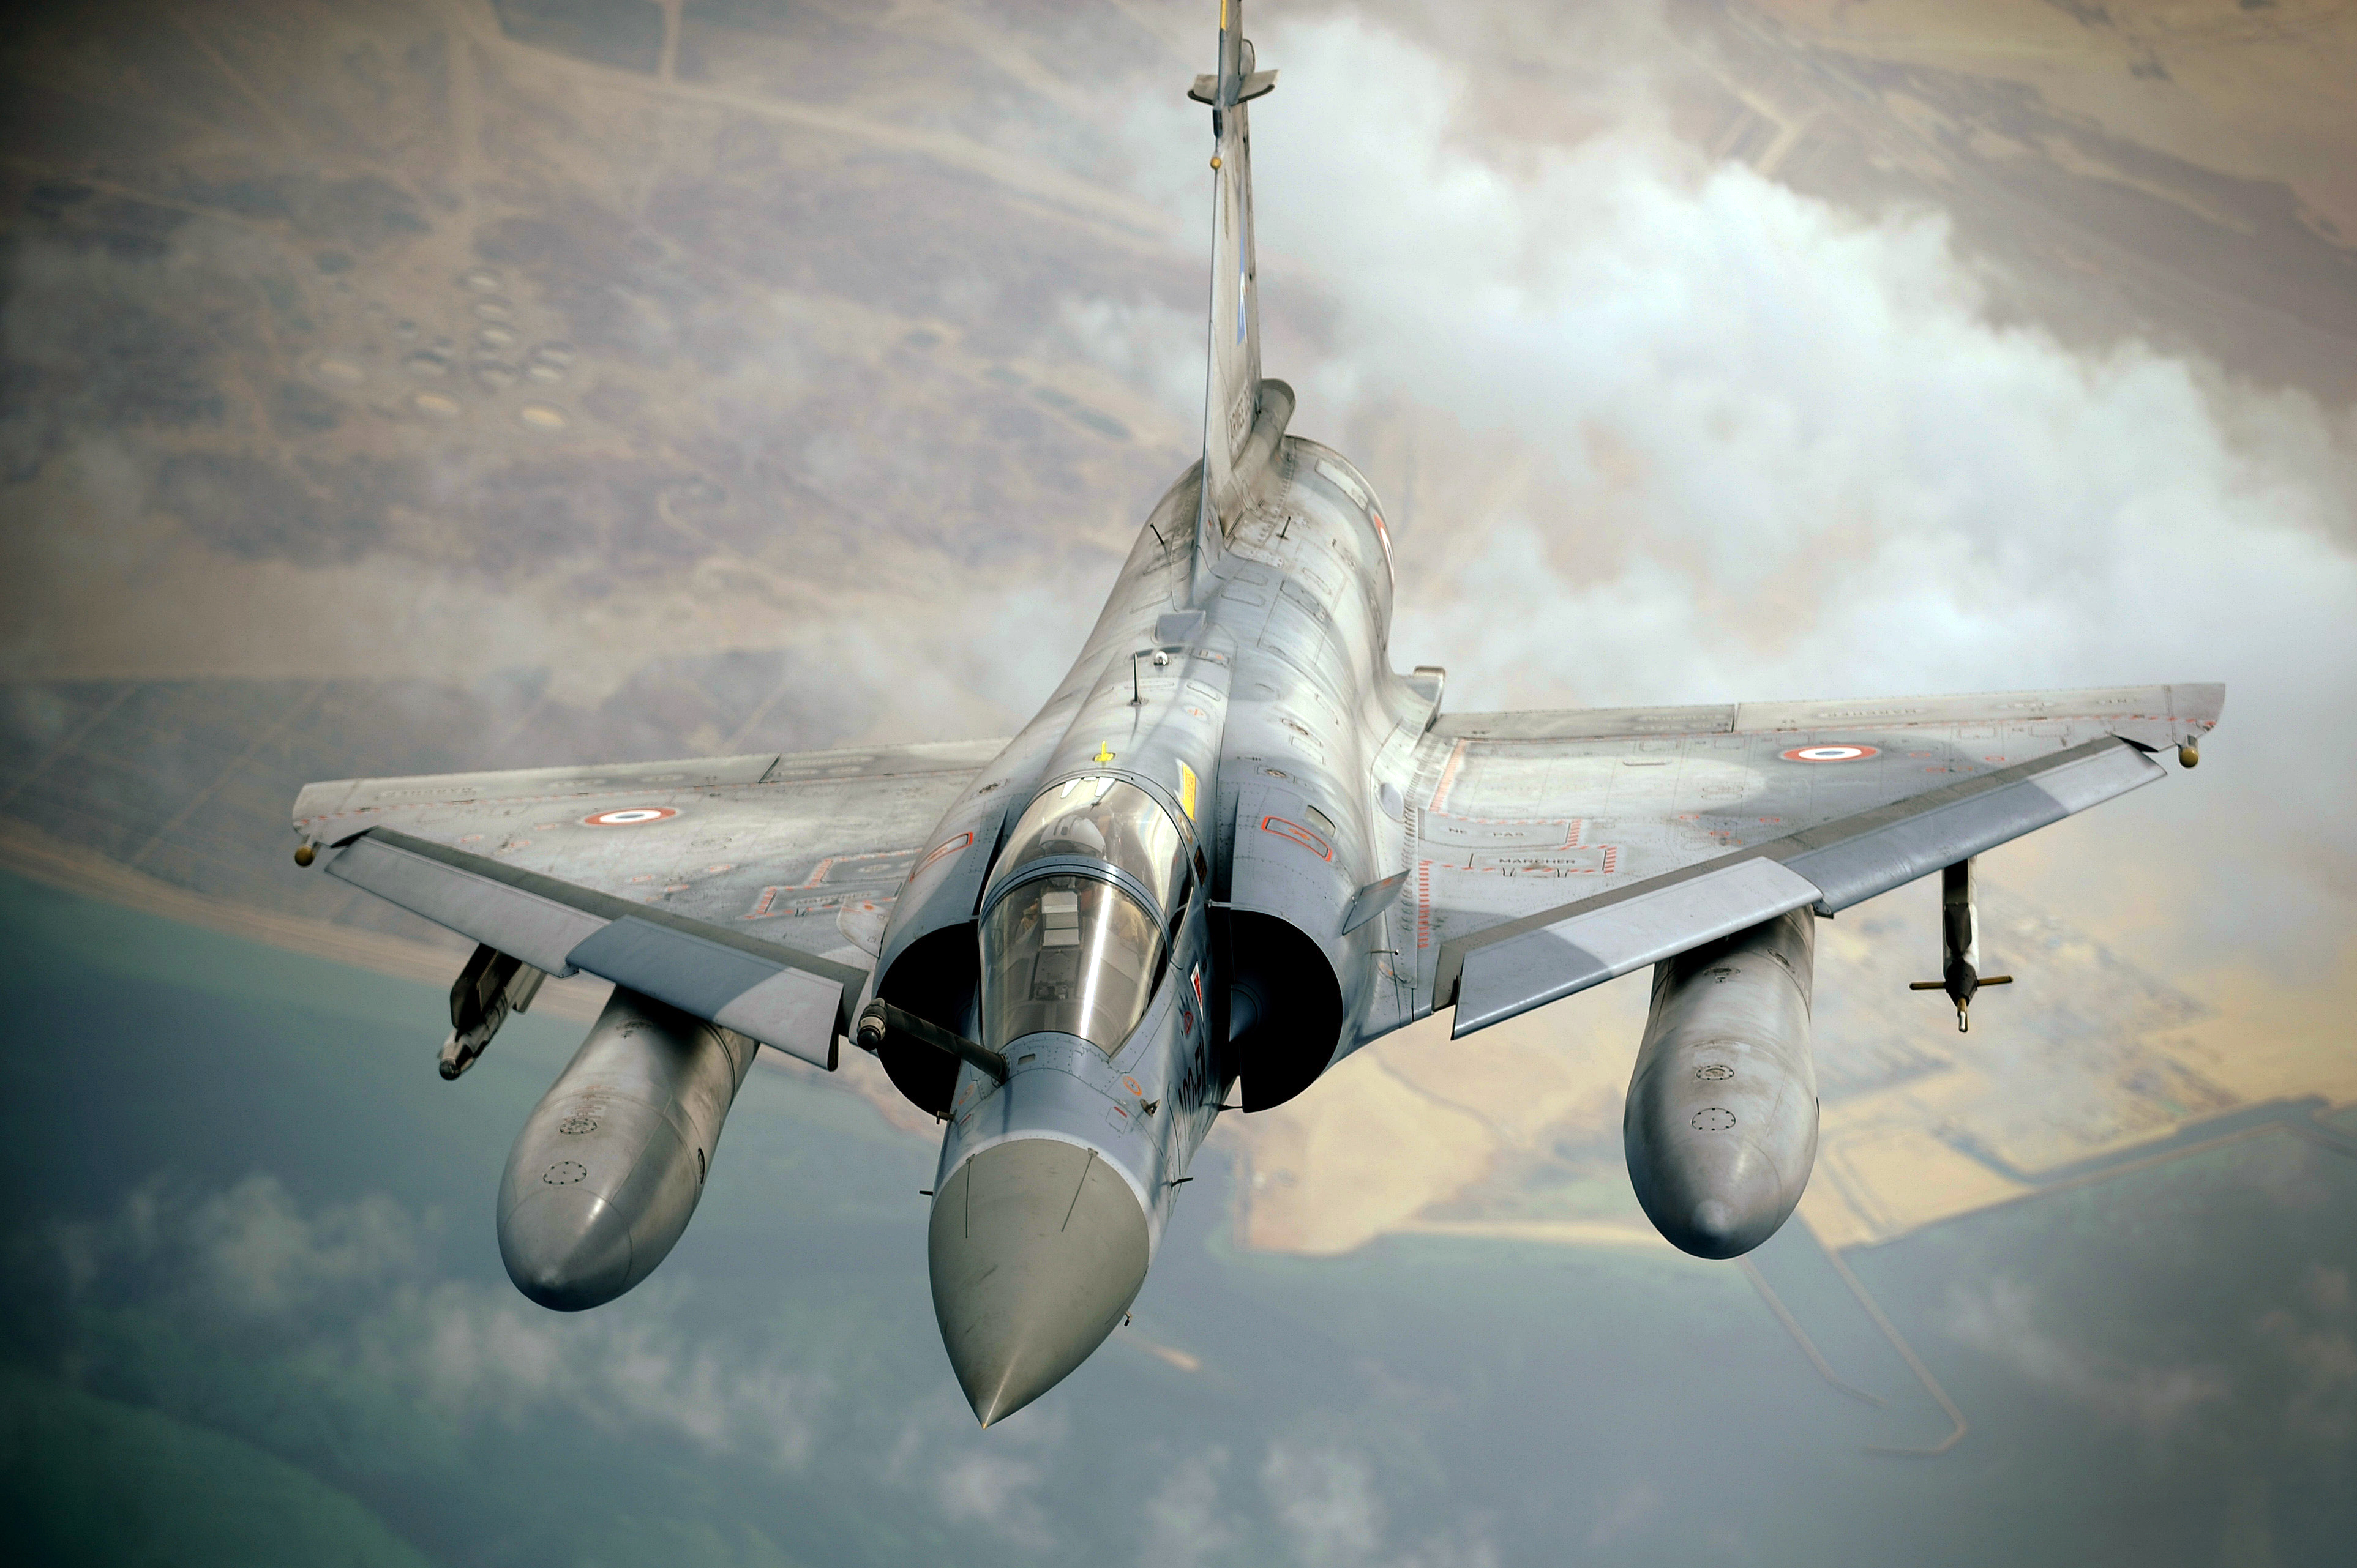
\includegraphics[width=1\linewidth]{img/mirage2000.jpg}
			\caption{The fleet of aircraft consists on Mirage 2000 (source: wikipedia; public domain)}
			\end{figure}

			A simplified description follows.

		    A series of $j \in \mathcal{J}$ missions are planned along a horizon divided into $t \in \mathcal{T}$ periods. Each mission requires a certain number $r_{j}$ of aircraft $i \in \mathcal{I}$ which it employs for a time duration defined by $h_j$ in each period. Set $a_{j} \subset \mathcal{I}$ lists the aircraft that can be assigned to each mission and set $O_i \subset \mathcal{J}$ consists of missions for which aircraft $i$ can be used.

		    Aircraft require recurrent preventive maintenance operations (of fixed duration $m$) since the realization of missions diminish their remaining flight hours. An aircraft cannot be used for a mission $j$ if its remaining flight hours are less than the amount $h_j$ required by mission $j$. A maintenance operation assigns each aircraft exactly $H$ flight hours. The remaining flight hours not used before the maintenance operation are lost. 


		\end{block}

	\end{column} % End of the first column

	\begin{column}{\sepwid}\end{column} % Empty spacer column

	\begin{column}{\twocolwid} % Begin a column which is two columns wide (column 2)

		\setbeamercolor{block alerted title}{fg=black,bg=norange} % Change the alert block title colors
		\setbeamercolor{block alerted body}{fg=black,bg=white} % Change the alert block body colors

	\begin{column}{\onecolwid}\end{column} % Empty spacer column

	\begin{column}{\twocolwid}
			\vspace*{-5ex}
			\begin{alertblock}{}				
				\begin{itemize}
					\item Doctorant (email): Franco Peschiera (franco.peschiera@isae-supaero.fr)
					\item Directeurs de Thèse: Olga Battaïa, Alain Haït, Nicolas Dupin
					\item Laboratoire, Université: ISAE-SUPAERO
					\item Collaboration industrielle: DGA
				\end{itemize}
			\end{alertblock}

	\end{column}

	\begin{column}{\onecolwid}\end{column} % Empty spacer column

		\begin{figure}
			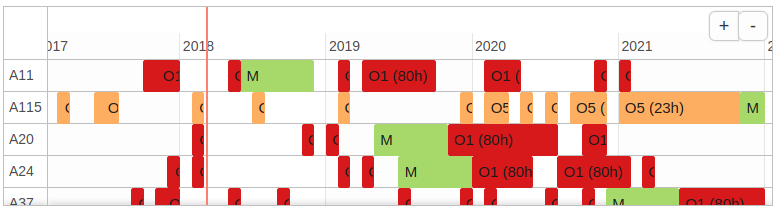
\includegraphics[width=1\linewidth]{img/calendar2.png}
			\caption{Partial solution showing the planning of maintenances (green) and assignments of missions (red and yellow) for some aircraft (in rows) over time periods (in columns).}
		\end{figure}

	\begin{columns}[t,totalwidth=\twocolwid] % Split up the two columns wide column

		\begin{column}{\twocolwid}\vspace{-.6in} % The first column within column 2 (column 2.1)

			\begin{block}{Mathematical model}

				The following model represents feasible and optimal solutions to the problem.

			    \begin{align*}
			    	& \text{Min}\; \sum_{t \in \mathcal{T}, i \in \mathcal{I}} m_{it} \times H - \sum_{i \in \mathcal{I}} rut_{i|\mathcal{T}|} \\
			        & \sum_{t' \in \mathcal{T}^{s}_t} \sum_{i \in \mathcal{I}} m_{it'} + N_t \leq M^{max}
			          & t \in \mathcal{T} \\
			        & \sum_{i \in \mathcal{I}_j} a_{jti} = R_j
			                & j \in \mathcal{J}, t \in \mathcal{T}_j  \\
			        & \sum_{t' \in \mathcal{T}^{s}_t} m_{it'} + \sum_{j \in \mathcal{J}_t \cap \mathcal{O}_i} a_{jti} \leq 1 
			                & t \in \mathcal{T}, i \in \mathcal{I}\\
			        & a^s_{jti} \geq a_{jti} - a_{j(t-1)i}
			                & j \in \mathcal{J}, t \in \mathcal{T}_j, i \in \mathcal{I}_j \\
			        & \sum_{t' \in \mathcal{T}^{MT}_{jt}} a^s_{jt'i} \leq a_{jti} 
			        & j \in \mathcal{J}, t \in \mathcal{T}_j, i \in \mathcal{I}_j \label{eq:start3}\\
			       & \sum_{t' \in \mathcal{T}^{s}_t} \sum_{i \in \mathcal{I}_k} m_{it'} \leq AK_{kt}
			        &k \in \mathcal{K}, t \in \mathcal{T} \\
			         & rut_{it} \leq rut_{i(t-1)} + H m_{it} \notag \\ 
			         	& - \sum_{j \in \mathcal{J}_t \cap \mathcal{O}_i} a_{jti} H_j 
			         	& t =1, ..., \mathcal{T}, i \in \mathcal{I} \\
			        & rut_{i0} = Rut^{Init}_i
			               & i \in \mathcal{I} \\
			        & rut_{it} \geq H m_{it}
			                & t \in \mathcal{T}, i \in \mathcal{I}\\ 
			        & rut_{it} \in [0,H]
			                & t \in \mathcal{T}, i \in \mathcal{I} \\
			        & m_{it'} + m_{it} \leq 1
			          & t \in \mathcal{T}, t' \in \mathcal{T}^{m}_t, i \in \mathcal{I}\\ 
			        & \sum_{t' \in \mathcal{T}^{M}_t} m_{it'} \geq  m_{it}
			          & t \in \mathcal{T}, i \in \mathcal{I}\\
			        & m_{it} = 0
			          & t \in \mathcal{T}^{m_{ini}}_i, i \in \mathcal{I} \\
			        & \sum_{t \in \mathcal{T}^{M_{ini}}_i} m_{it} \geq  1 
			          & i \in \mathcal{I}
			    \end{align*}

			\end{block}

			\setbeamercolor{block alerted title}{fg=white,bg=dblue!70} % Colors of the highlighted block titles
			\setbeamercolor{block alerted body}{fg=black,bg=dblue!10} % Colors of the body of highlighted blocks

			\begin{alertblock}{Acknowledgements}
					
				This thesis is half financed by DGA and takes place at ISAE-SUPAERO.

			\end{alertblock}

		\end{column} % End of column 2.1

		\end{columns} % End of the split of column 2

	\end{column} % End of the second column



	\begin{column}{\sepwid}\end{column} % Empty spacer column

	\begin{column}{\onecolwid} % The third column

			% \begin{column}{\onecolwid}\vspace{-.6in} %  (column 2.2)

			\begin{block}{Results}

				The following figures show some views on the output generated by the model.

				\begin{figure}
					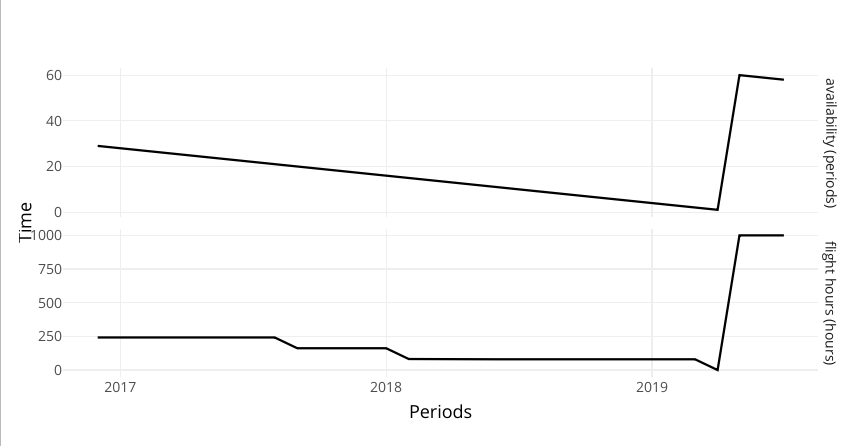
\includegraphics[width=1\linewidth]{img/remaining2.png}
					\caption{Partial solution showing the remaining periods and flight hours for a single aircraft. Both values should ideally reach 0 at the same time.}
					% \label{rem}
				\end{figure}	


				\begin{figure}
					
					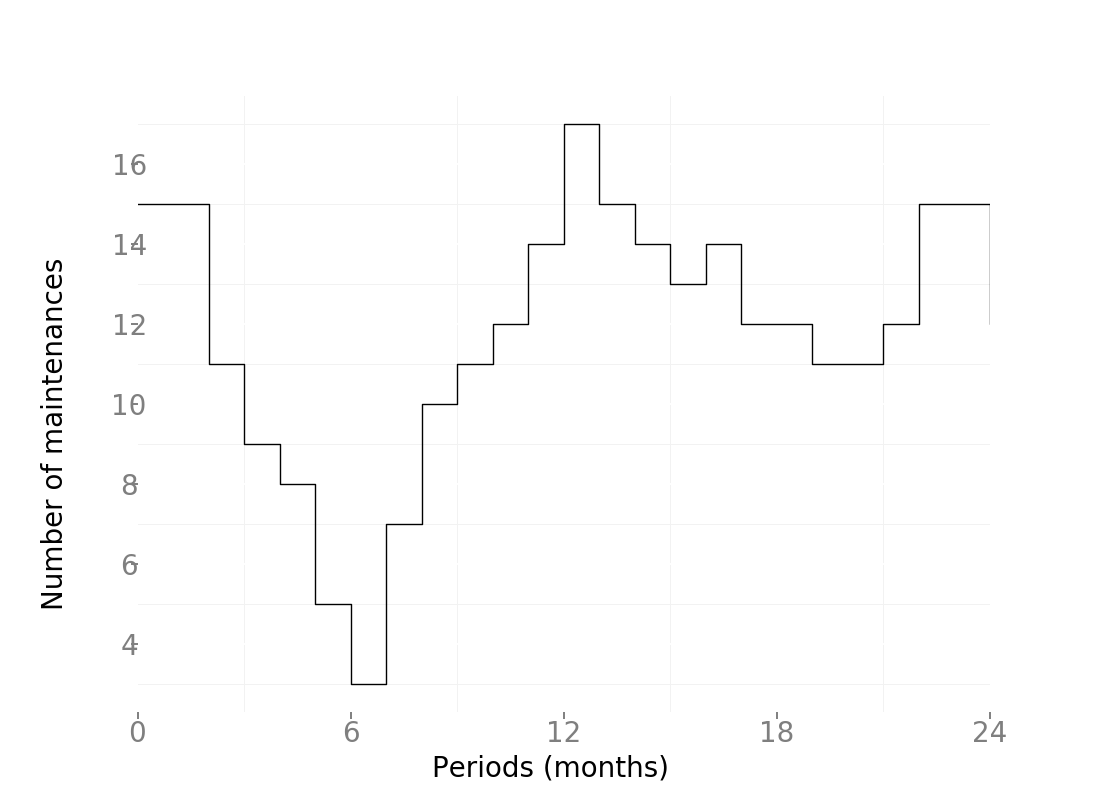
\includegraphics[width=1\linewidth]{img/num-maintenances.png}
					\caption{Partial solution showing the total number of aircraft under maintenance at each period. This value should be as constant (and low) as possible.}
					% \label{maint}
				\end{figure}
			\end{block}

			% \end{column} % End of column 2.2

		%----------------------------------------------------------------------------------------
		%	CONCLUSION
		%----------------------------------------------------------------------------------------
		\begin{block}{Discipline and techniques}
			
			\textbf{Operations Research}
			
			\begin{itemize}
				\item Commonly called "The science of better".
				\item Consists of techniques to help the decision making process.
				\item Used for planning, programming, scheduling, routing, pricing in production, logistics, human resources, marketing and investment.
			\end{itemize}
			
			\textbf{Mathematical programming}

			\begin{itemize}
				\item Permits the modelling of a problem as a set of variables and equations.
				\item Solved via dedicated software optimized to solve this kinds of equations.
				\item Used by the industry and governments to solve real-life large-scale problems all over the world.
			\end{itemize}

		\end{block}

	%----------------------------------------------------------------------------------------

	\end{column} % End of the third column

\end{columns} % End of all the columns in the poster

% \begin{columns}[t]

% 	\begin{column}{\onecolwid}
% 		
\includegraphics[width=1\linewidth]{img/AFIS_logo.jpg}
% 	\end{column} % Empty spacer column

% 	\begin{column}{\onecolwid}\end{column}
% 	\begin{column}{\threecolwid}
% 			Séminaire Doctoral, Rencontres académie – industrie AFIS\\
% 			5-6 décembre 2018, Université de Lorraine
% 	\end{column}

% \end{columns}

\end{frame} % End of the enclosing frame

\end{document}
